\qcor targets an execution model whereby application execution is directed by the host with access to an attached quantum device. Applications are broadly thought of as containing two components: a main, classical part, and one or more quantum kernels or subroutines. Figure \ref{fig:exec_model} illustrates \qcor's execution model. Designated quantum kernels are compiled and offloaded to the quantum device. The quantum device executes \qcor library calls and/or \qcor regions identified by directive notations. When the host encounters a quantum kernel, the quantum kernel, in the form of compiled hardware native or simulator 
instructions, is passed to the quantum device controller. Execution on the host is asynchronous to execution on the quantum device. 
Currently, \qcor exposes initialization, synchronization, execution and memory management library \ac{API} to the user that enable a wide variety of hybrid quantum-classical use cases.

\begin{figure*}
 \centering
 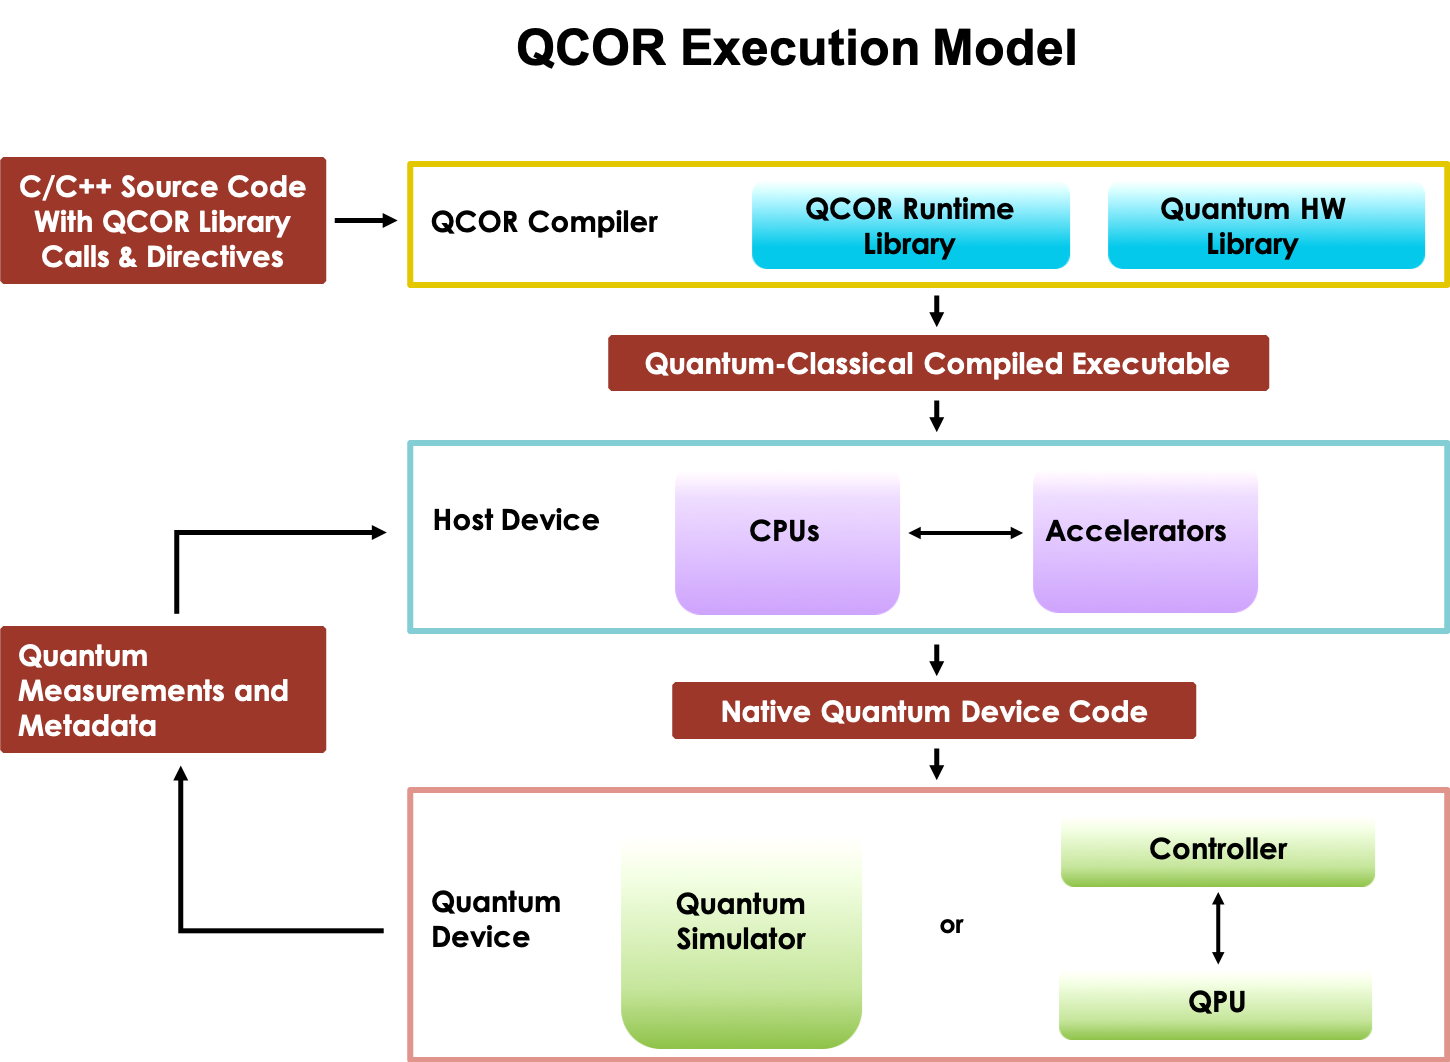
\includegraphics[width=5in,height=4in]{figures/Execution_Model_Illustration_v3.png}
  \caption{Diagram of \qcor Execution Model}
  \label{fig:exec_model}
\end{figure*}

